\documentclass{beamer}
\usepackage[spanish]{babel}
\usepackage[utf8]{inputenc}
\usepackage{graphicx}
\graphicspath{ {./images/}}

\usetheme{Madrid}
\usecolortheme{default}

%------------------------------------------------------------
%This block of code defines the information to appear in the
%Title page
  \title[PC3 Estadística Aplicada] %optional
{Aplicación de tests no paramétricos}

\subtitle{
  Caso: Distribucion de notas de estudiantes de la academia
    Trilce en los ultimos 3 años
}

\author % (optional)
{
  Alvarez \and Bautista \and Burga, Ever \and
  Casanova, Italo \and  Cuyate, Brayan
}

\institute
{
  Facultad de Ingenieria Industrial y de Sistemas\\
  \textbf{Universidad Nacional de Ingenieria}
}

\date
{Diciembre 2022}

% \logo{\includegraphics[height=1cm]{overleaf-logo}}

%End of title page configuration block
%------------------------------------------------------------

%------------------------------------------------------------
%The next block of commands puts the table of contents at the
%beginning of each section and highlights the current section:

\AtBeginSection[]
{
  \begin{frame}
    \frametitle{Tabla de Contenido}
    \tableofcontents[currentsection]
  \end{frame}
}
%------------------------------------------------------------


\begin{document}

%The next statement creates the title page.
\frame{\titlepage}


%---------------------------------------------------------
%This block of code is for the table of contents after
%the title page
\begin{frame}
\frametitle{Tabla de Contenido}
\tableofcontents
\end{frame}
%---------------------------------------------------------
\section{Objetivos}

%---------------------------------------------------------
\begin{frame}

\frametitle{Objetivos del trabajo}

\begin{alertblock}{General}
  Determinar si el ciclo de repaso ha sido útil para los postulantes a la
  Universidad Nacional de Ingenieria en la academia Trilce
\end{alertblock}
\end{frame}

\begin{frame}
\frametitle{Objetivos especificos}

\begin{columns}
\column{0.5\textwidth}

  \begin{itemize}
      \item Probar si alguna de las medianas de la distribución del examen general del 6 de enero de 2020
      de acuerdo a sede difiere con un nivel de significancia del 5\% con la prueba de Kruskal-Wallis.
      \item Comparar el desempeño de los estudiantes antes de tomar un ciclo
        de repaso y despues de este.
      \item Comparar la evolucion del desempeño de aquellos que tomaron más de un simulacro.

  \end{itemize}

\column{0.5\textwidth}

  \begin{itemize}
      \item Comparar la potencia entre el test de \textit{Wilcoxon} y
      el \textit{Test de signos}
  \end{itemize}
\end{columns}
\end{frame}

%---------------------------------------------------------

\begin{frame}
\frametitle{Hipotesis especificas}
  \begin{itemize}
      \item Las personas que trabajan una cantidad de horas superior a
        la media tienen una mejor destribucion de ingresos que aquellas
        que no lo hacen
      \item Las personas de mediana edad poseen una mejor distribucion
        de ingreso que las personas jovenes
      \item El promedio de ingresos de la poblacion mexicana es mayor
        que la peruana
  \end{itemize}

\end{frame}

%---------------------------------------------------------
\section{Metodología y Resultados}

\begin{frame}
    \frametitle{Test de Kruskal-Wallis}
    % import image with a description
    La distribución de las notas de los estudiantes de la academia Trilce
    de acuerdo a sede es la siguiente: 
    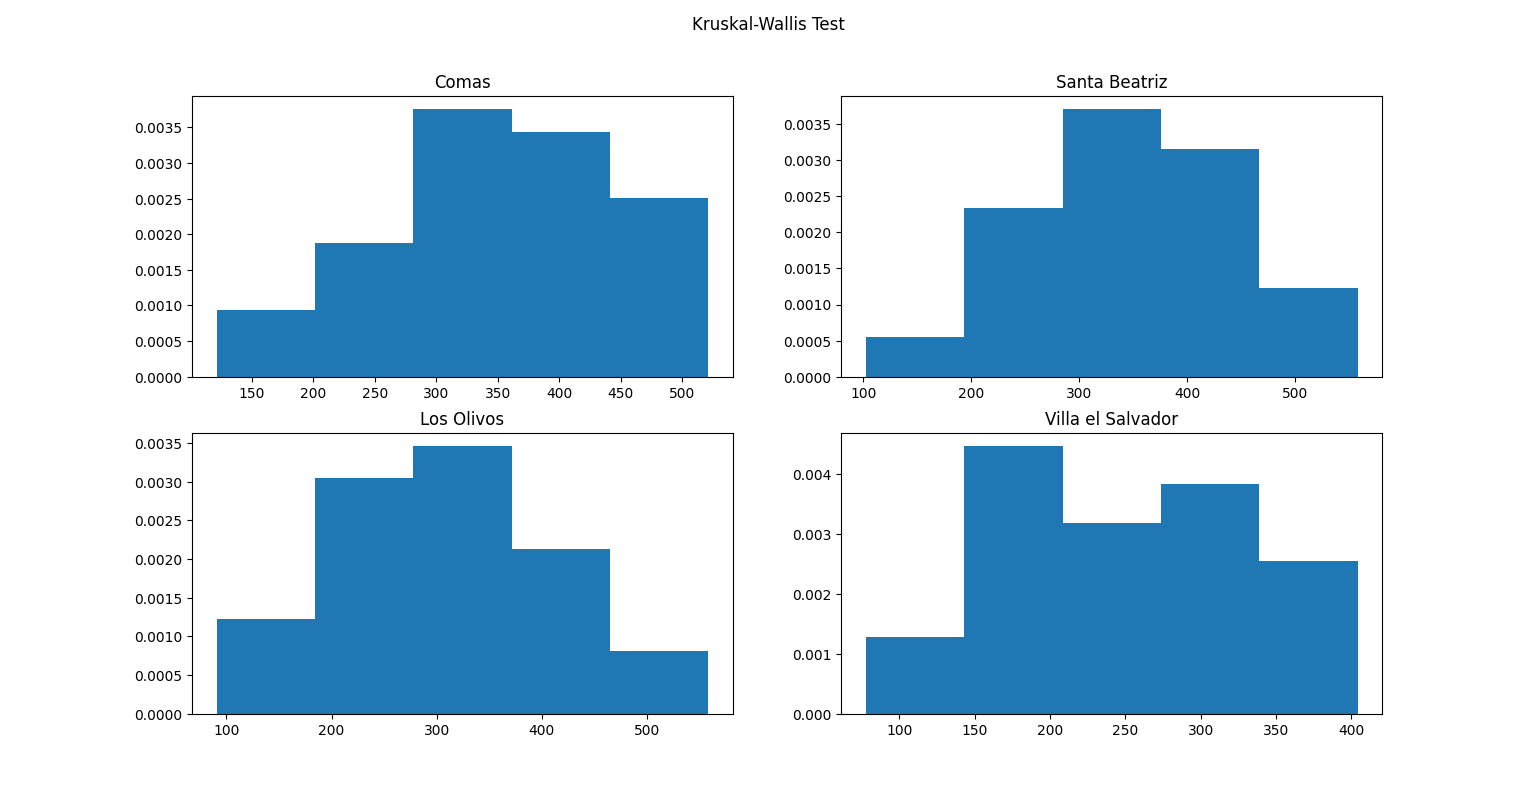
\includegraphics[width=1\textwidth]{cap/images/kruskal.png}
\end{frame}

\begin{frame}
    \frametitle{Test de Kruskal-Wallis}
    % import image with a description
    Con un gráfico de cajas se puede observar que la distribución de 
    Villa el Salvador tiene una mediana muestral que es distinta a las demás. 
    \centering
    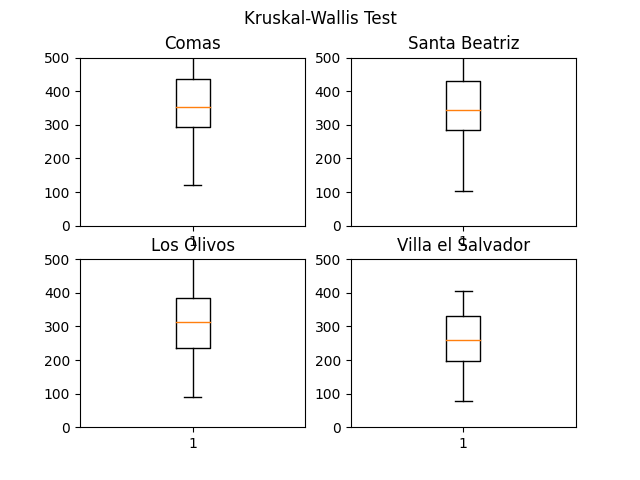
\includegraphics[width=0.8\textwidth]{cap/images/kruskal_boxplot.png}
\end{frame}

\begin{frame}
    \frametitle{Test de Kruskal-Wallis}
    % import image with a description
    \begin{itemize}
        \item Sea la hipótesis nula $H_0$ es que las distribuciones de las notas de los estudiantes de la academia Trilce de acuerdo a sede son iguales.
        \item La hipótesis alternativa $H_1$ es que al menos una de las distribuciones es distinta.
    \end{itemize}
    \begin{itemize}
        \item La prueba de Kruskal-Wallis arroja los siguientes resulados:
        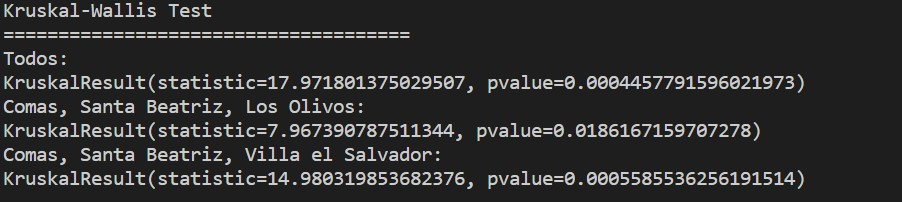
\includegraphics[width=0.8\textwidth]{cap/images/resultados_kruskal.jpg}
        \item Se rechaza $H_0$ y se concluye que al menos alguna distribución de notas de los estudiantes de la academia Trilce de acuerdo a sede difiere con un nivel de significancia del 5\%
    \end{itemize}
\end{frame}

\begin{frame}
    \frametitle{Test de Kruskal-Wallis}
    % import image with a description
    Al comparar las cuatro distribuciones el p-value es 0.000445. 
    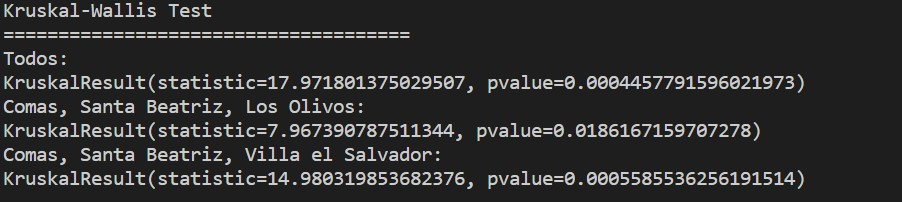
\includegraphics[width=0.8\textwidth]{cap/images/resultados_kruskal.jpg}
    
    Sin embargo, un detalle que resalta es que al excluir la distribución de Villa el Salvador, el p-value es 0.0186.
    Este valor sería significativo para un nivel de confianza del 1\% y señala una posible 
    diferencia que consideramos que es susceptible de futura investigación.
    
\end{frame}

\begin{frame}
  \frametitle{Test de Signos}


\end{frame}

\begin{frame}
  \frametitle{Test de Wilcoxon}

  Si bien, el test de signos puede cumplir la misma funcion que el de
  \textbf{Wilcoxon}, este ultimo tiene mayor potencia al momento de
  detectar diferencia de medias.


\end{frame}

%---------------------------------------------------------


\section{Conclusiones}

\begin{frame}
  \frametitle{Hipotesis 1}
  

\end{frame}


\begin{frame}

  \frametitle{Otras conclusiones}

\end{frame}

\end{document}
